\documentclass[notitlepage]{svjour3}

\usepackage{graphics}
\usepackage{graphicx}
\usepackage[utf8]{inputenc}
\usepackage[T1]{fontenc}
\usepackage[american]{babel}
\usepackage{pgfplots}
\usepackage{amsmath}
\usepackage{tikz}
\usepackage{csquotes}
\usepackage{booktabs} % For formal tables.
\usepackage{authblk}
\usepackage{blkarray}
\usepackage{subcaption} % For subfigures.
\captionsetup{compatibility=false} % For subcaption.
\usepackage{tabularx}

\newtheorem{thm}{Theorem}[section]
\newtheorem{cor}[thm]{Corollary}
\newtheorem{lem}[thm]{Lemma}
\newtheorem{asp}{Assumption}%[section]
\newtheorem{defin}{Definition}[section]
\newtheorem{prop}{Proposition}[section]
\newtheorem{rem}{Remark}[section]
\newtheorem{alg}{Algorithm}[section]
\newtheorem{conj}{Conjecture}[section]
\newtheorem{comment}{Comment}[section]

\newcommand{\ind}[1]{1\hspace{-0.125cm}1\{#1\}}
\newcommand{\CR}{ {\mbox{\em CR}} }
\newcommand{\mv}{ {\mbox{v}} }

\newcommand{\SA}{ {\cal A} }
\newcommand{\SB}{ {\cal B} }
\newcommand{\SC}{ {\cal C} }
\newcommand{\SD}{ {\cal D} }
\newcommand{\SE}{ {\cal E} }
\newcommand{\SF}{ {\cal F} }
\newcommand{\SG}{ {\cal G} }
\newcommand{\SH}{ {\cal H} }
\newcommand{\SI}{ {\cal I} }
\newcommand{\SJ}{ {\cal J} }
\newcommand{\SK}{ {\cal K} }
\newcommand{\SL}{ {\cal L} }
\newcommand{\SM}{ {\cal M} }
\newcommand{\SN}{ {\cal N} }
\newcommand{\SO}{ {\cal O} }
\newcommand{\SP}{ {\cal P} }
\newcommand{\SQ}{ {\cal Q} }
\newcommand{\SR}{ {\cal R} }
\newcommand{\sS}{ {\cal S} }
\newcommand{\ST}{ {\cal T} }
\newcommand{\SU}{ {\cal U} }
\newcommand{\SV}{ {\cal V} }
\newcommand{\SW}{ {\cal W} }
\newcommand{\SX}{ {\cal X} }
\newcommand{\SY}{ {\cal Y} }
\newcommand{\SZ}{ {\cal Z} }
 
\newcommand{\bA}{ {\bf A} }
\newcommand{\bB}{ {\bf B} }
\newcommand{\bC}{ {\bf C} }
\newcommand{\bD}{ {\bf D} }
\newcommand{\bE}{ {\bf E} }
\newcommand{\bF}{ {\bf F} }
\newcommand{\bG}{ {\bf G} }
\newcommand{\bH}{ {\bf H} }
\newcommand{\bI}{ {\bf I} }
\newcommand{\bJ}{ {\bf J} }
\newcommand{\bK}{ {\bf K} }
\newcommand{\bL}{ {\bf L} }
\newcommand{\bM}{ {\bf M} }
\newcommand{\bN}{ {\bf N} }
\newcommand{\bO}{ {\bf O} }
\newcommand{\bP}{ {\bf P} }
\newcommand{\bQ}{ {\bf Q} }
\newcommand{\bR}{ {\bf R} }
\newcommand{\bS}{ {\bf S} }
\newcommand{\bT}{ {\bf T} }
\newcommand{\bU}{ {\bf U} }
\newcommand{\bV}{ {\bf V} }
\newcommand{\bW}{ {\bf W} }
\newcommand{\bX}{ {\bf X} }
\newcommand{\bY}{ {\bf Y} }
\newcommand{\bZ}{ {\bf Z} }
 
\newcommand{\mb}[1] { {\mbox{\rm #1}} }
\newcommand{\ee}{ {\mbox{e}} }
\newcommand{\diag}{ {\mbox{diag}} }
\newcommand{\bGamma}{ {\mbox{\boldmath $\Gamma$}} }
\newcommand{\bLambda}{ {\mbox{\boldmath $\Lambda}} }
\newcommand{\bOmega}{ {\mbox{\boldmath $\Omega$}} }
\newcommand{\bUpsilon}{ {\mbox{\boldmath $\Upsilon$}} }
\newcommand{\bPi}{ {\mbox{\boldmath $\Pi$}} }
\newcommand{\bPsi}{ {\mbox{\boldmath $\Psi$}} }
\newcommand{\bpi}{ {\mbox{\boldmath $\pi$}} }
\newcommand{\bphi}{ {\mbox{\boldmath $\phi$}} }
\newcommand{\bpsi}{ {\mbox{\boldmath $\psi$}} }
\newcommand{\balpha}{ {\mbox{\boldmath $\alpha$}} }
\newcommand{\bbeta}{ {\mbox{\boldmath $\beta$}} }
\newcommand{\bdelta}{ {\mbox{\boldmath $\delta$}} }
\newcommand{\bepsilon}{ {\mbox{\boldmath $\epsilon$}} }
\newcommand{\blambda}{ {\mbox{\boldmath $\lambda$}} }
\newcommand{\bgamma}{ {\mbox{\boldmath $\gamma$}} }
\newcommand{\bomega}{ {\mbox{\boldmath $\omega$}} }
\newcommand{\btau}{ {\mbox{\boldmath $\tau$}} }
\newcommand{\bnu}{ {\mbox{\boldmath $\nu$}} }
\newcommand{\bvarep}{ {\mbox{\boldmath $\varepsilon$}} }

\newcommand{\bxi}{ {\mbox{\boldmath $\xi$}} }
\newcommand{\bzeta}{ {\mbox{\boldmath $\zeta$}} }
\newcommand{\bvarphi}{ {\mbox{\boldmath $\varphi$}} }
\newcommand{\bkappa}{ {\mbox{\boldmath $\kappa$}} }
\newcommand{\bsigma}{ {\mbox{\boldmath $\sigma$}} }
\newcommand{\brho}{ {\mbox{\boldmath $\rho$}} }
\newcommand{\bvarrho}{ {\mbox{\boldmath $\varrho$}} }
\newcommand{\bPhi}{ {\bf \Phi} }

\newcommand{\boo}{ {\bf 0} }
\newcommand{\bzr}{ {\bf 0} }
\newcommand{\bon}{ {\bf 1} }
\newcommand{\ba}{ {\bf a} }
\newcommand{\bb}{ {\bf b} }
\newcommand{\bc}{ {\bf c} }
\newcommand{\bd}{ {\bf d} }
\newcommand{\be}{ {\bf e} }
\newcommand{\bff}{ {\bf f} }
\newcommand{\boldf}{ {\bf{f} } }
\newcommand{\bg}{ {\bf g} }
\newcommand{\bh}{ {\bf h} }
\newcommand{\bi}{ {\bf i} }
\newcommand{\bj}{ {\bf j} }
\newcommand{\bk}{ {\bf k} }
\newcommand{\bl}{ {\bf l} }
\newcommand{\bm}{ {\bf m} }
\newcommand{\bn}{ {\bf n} }
\newcommand{\bo}{ {\bf o} }
\newcommand{\bp}{ {\bf p} }
\newcommand{\bq}{ {\bf q} }
\newcommand{\br}{ {\bf r} }
\newcommand{\bs}{ {\bf s} }
\newcommand{\bt}{ {\bf t} }
\newcommand{\bu}{ {\bf u} }
\newcommand{\bv}{ {\bf v} }
\newcommand{\bx}{ {\bf x} }
\newcommand{\bw}{ {\bf w} }
\newcommand{\by}{ {\bf y} }
\newcommand{\bz}{ {\bf z} }

\providecommand{\keywords}[1]{\textbf{\textit{Keywords:}} #1}

\begin{document}

\title{P-score: a Reputation Bibliographic Index that Complements Citation Counts} 

\author{
 João Mateus de Freitas Veneroso \and
 Marlon Dias \and
 Berthier Ribeiro-Neto \and
 Nivio Ziviani \and
 Edmundo de Souza e Silva
}

\institute{
 João Mateus de Freitas Veneroso \at
 Universidade Federal de Minas Gerais, Av. Pres. Antônio Carlos, 6627 - Pampulha, Belo Horizonte - MG, 31270-901,
 Departamento de Ciência da Computação, Sala 4304 \\
 Tel.: +55 (31) 99436-0909 \\
 \email{jmfveneroso@gmail.com} \and
 Marlon Dias              \at Universidade Federal de Minas Gerais \and
 Berthier Ribeiro-Neto    \at Universidade Federal de Minas Gerais \and
 Nivio Ziviani            \at Universidade Federal de Minas Gerais \and
 Edmundo de Souza e Silva \at Universidade Federal do Rio de Janeiro
}

\authorrunning{J. M. F. Veneroso, M. Dias, B. Ribeiro-Neto, N. Ziviani, and E. S. Silva} % if too long for running head

% \providecommand{\keywords}[1]{\textbf{\textit{Index terms---}} #1}

\maketitle

% \textbf{Declarations of interest: none} \\
\textbf{Conflict of Interest: The authors declare that they have no conflict of interest.} \\
% \\
% \\
% \textbf{Corresponding author:} \\
% João Mateus de Freitas Veneroso \\
% Mailing address: Universidade Federal de Minas Gerais, Av. Pres. Antônio Carlos, 6627 - Pampulha, Belo Horizonte - MG, 31270-901 \\
% Tel: +55 (31) 99436-0909 \\
% Email: jmfveneroso@gmail.com \\

\begin{abstract}
The notions of reputation and popularity in academia are critical for taking 
decisions on research grants, faculty position tenure, and research excellence awards. 
These notions are almost always associated with the publication track 
records of the researchers. Thus, it is important to assess 
publication track records quantitatively. To quantify a publication record, 
bibliographic indices are usually adopted. Among these, citation-based indices
such as the H-index are frequently considered. 
In this paper we study the correlation between P-score, a publication record index
and H-index, the most popular citation-based index. 
While H-indices reflect the popularity of a given
publication or researcher in academia, P-scores reflect the reputation of a publication or
researcher among its peers. Popularity and reputation are frequently considered 
to be equivalent properties, however they are not identical. Indeed, 
we first show that H-indices and P-scores are correlated with a Kendall-Tau coefficient 
that exceeds 0.5. However, we also notice that they have important differences. 
Particularly, we identify publication venues with high H-indices and low 
P-scores, as well as venues with low H-indices and high P-scores. We provide interpretations 
for these findings and discuss how they can be used by research funding councils and committees
to better support their funding decisions.
\end{abstract}

\keywords{P-score \and H-index \and Bibliographic Index \and Reputation Flows}

\section{Introduction}
\label{sec:introduction}

Academic research evaluation is a topic of interest to universities, research groups,
research funding institutions, and the public at large. It is used to decide laboratory space
allocation, research grants, tenure track, university choice by students, and more. It also 
has a direct impact on the reputation of the university or institution, which
affects the ability of the institution to attract the best possible talent. While evaluation of
academic research is complex, usually a function of multiple variables, a dominant variable in
most evaluation procedures is the research output of the institution. In particular, considerable
emphasis is given to the papers published by the professors and students of the institution, as
well as the quality of these papers in terms of their impact on scientific knowledge. A rather
popular approach to evaluate publication impact is to compare journals, conferences or papers
through the usage of academic impact indicators. A popular and moderately effective approach is to
compute an index based on the number of citations received by a given piece of research and
assume that the number of citations is a good proxy for research quality. However,
this approach has multiple shortcomings. 

First, in the evaluation and bibliometrics research communities, citations are understood
as a measure of attention rather than a proxy for impact or quality. Citations measure 
the attention to a paper of peers in related fields \cite{Loach2015}, not the quality of the 
work produced. Second, citations can take a long time to happen. To illustrate this, in a recent
study that looked at first time to citation in a universe of more than a million papers, half the 
papers only received their first citation 20 months or more after they were
published~\cite{Nane2012}. Third, citations are not simple to compute and are not always broadly
available, particularly at the level of individual researchers.

Despite these limitations, citation-based indices continue to be a popular approach to
academic research evaluation~\cite{Kellner2008}.
Nonetheless, it is desirable to employ
complementary indicators that tackle the exposed problems without loss of effectiveness.

Academic reputation is an individual or group property strongly associated with 
academic impact, and while being similar it is not identical to academic popularity. An 
actor's popularity depends solely on the the total number of endorsements
the actor receives from other actors, while its reputation or prestige depends on the 
reputations of the endorsing actors~\cite{Bollen2006}. Reputable venues tend to 
concentrate the most relevant research papers 
because that is how they acquire and keep their good reputations. At the same time, 
reputable authors seek to publish on reputable venues because it gives their 
research more visibility and accreditation. Therefore, researchers convey reputation
to a venue proportionally to their own reputation and the reputation of researchers
is proportional to the reputation of the venues where they publish.
This relationship between authors and venues constitutes a reputation network in which 
authors influence venue reputations and vice versa. 

{\em P-score}~\cite{Ribas2015a} is a graph-based modeling index that attributes quantitative
reputations to venues based on the publication patterns of a reference group of researchers,
without relying on citation information. It deals with the three problems discussed previously. 

First, instead of measuring the amount of researcher attention, P-score measures reputations
which, under certain assumptions, provide a better proxy for academic impact as was shown by 
Ribas et al.~\cite{Ribas2015a}. Second, while citations can take years to happen, reputations 
tend to be established earlier on. As a consequence, the quality of new research can be 
promptly estimated using P-scores computed on the newest publication data. Third, P-scores do
not require citation data to be computed, which means that they can be recomputed quickly whenever one finds fit or convenient.

Our interpretation of these results are based on the intuition that while H-indices provide a 
quantification of the popularity of a publication or researcher among their peers, P-scores 
provide a quantification of the reputation of a publication or researcher among peers. When
P-scores and H-indices are strongly correlated, we have venues that are popular and of high
reputation or unpopular with a low reputation. Second, when P-scores are high (better rank position) 
and H-indices are low (worse rank position) we have venues of good reputation
that are associated with small research communities or subareas and are accordingly less popular. Third, when P-scores
are low (worse rank position) and H-indices are high (better rank position) we have venues of good popularity 
(usually associated with large research communities) that do not have
a high reputation (in the sense that the reference group of researchers does not publish frequently there).

\section{Related Work}\label{sec:related-work}

Quantitative measures of scientific impact have a long history. An influential approach is
Garfield's Impact Factor~\cite{Garfield1955a}, a journal-level measure that is defined
by the mean number of citations received by articles published in a given journal over a 2-year period. 
Despite being one of the earliest approaches at measuring scientific impact, it has showed remarkable 
survivability. 
Pinski et al. \cite{Pinski1976} describe several limitations with the Impact Factor. Impact factors also suffered 
criticism for being misleading~\cite{Nature2016,Saha2003} and for lacking reliable validation from an independent 
audit~\cite{Rossner2007}. Riikonen et al. \cite{Riikonen2008} showed that actual citation 
and publication counts were better predictors of a scientist's contribution than impact factors in a 
study that assessed the scientific contribution of Finnish researchers in biomedicine.

The acceptance rate is another important journal-level indicator that attempts to quantify scientific impact. It
is defined by the proportion of accepted papers relative to the number of submitted papers. Chen et al. \cite{Chen2010} 
have shown that highly selective conferences, the ones having low acceptance rates, have higher 
scientific impact measured in terms of the number of citations received by the published papers.

The H-index is an author-level index proposed by Hirsch~\cite{Hirsch2005}. Since its formulation, it has been 
widely adopted as a measure of individual scientific research output.
The H-index takes into account both the number of publications and the number of citations per publication, 
achieving higher values when a researcher obtains a consistently high number of citations over multiple publications. 
The H-index has been criticized for not taking into account field specific citation
statistics~\cite{Wendl2007}. The G-index, proposed by Egghe~\cite{Egghe2006}, is a less strict variation 
of the H-index.

Citation counts and derived measures are straightforward to calculate, but they represent only a coarse
estimate of academic impact, because they are essentially popularity measures. Some people are popular but not 
prestigious and vice versa. For example, an author of pulp detectives may sell many books, but may not have earned 
the respect of literary critics as pointed by Bollen et al.~\cite{Bollen2006}. Citations from 
prestigious journals are more relevant than citations from peripheral journals, as noted by Pinski et al.~\cite{Pinski1976}. To address this issue, some studies distinguish popularity from 
reputation or prestige with the usage of citation weighting strategies~\cite{Ding2011,Yan2011a} or 
Page Rank based methods~\cite{Bollen2006,Sun2007}. 
Furthermore, Piwowar~\cite{Piwowar2013} noted that citation-based indices are slow, since the 
first citation to a scientific article can take years to happen, concluding that the development of 
alternative indices to complement citation analysis is not only desirable, but a necessity.
As discussed by Leydesdorff~\cite{Leydesdorff2009}, each indicator has advantages and disadvantages 
deriving from their inherent biases.

Martins et al. \cite{Martins2009} proposed a method of assessing the quality of scientific conferences 
through a machine learning classifier that makes use of multiple features in addition to citations.
Gonçalves et al.~\cite{Goncalves2014} quantified the impact of various features on a 
scholar's popularity. They concluded that, even though most of the considered features are strongly correlated 
with popularity, only two features are needed to explain almost all the variation in popularity between different 
researchers: the number of publications and the average quality of the scholar’s publication venues. 

The idea of reputation, without the direct use of citation data, was discussed by Nelakuditi et al.~\cite{Nelakuditi2011}. 
They proposed a measure called \textit{peers' reputation} for 
research conferences and journals, which ties the selectivity of the publication venue based upon 
the reputation of its authors' institutions. The proposed measure was shown to be a better indicator 
of the selectivity of a research venue than the acceptance ratio.

\section{P-score: a network-based index} 
\label{pscore} 

Contrary to citation counts such as the Impact 
Factor~\cite{Garfield1955a,Saha2003,Thomson2017,Balaban2012} and 
H-index~\cite{Benevenuto2016,Bar-Ilan2008,Egghe2008,Bornmann2005,Bornmann2011}, 
P-scores are a graph-based modeling index that takes into account 
the relations among researchers, papers they published and their publication venues. They are based on a framework of \textit{reputation flows}~\cite{Ribas2015} which we describe in this section.

Let a \emph{reputation graph} be a graph with three node types of academic entities: (a) {\em reputation sources} representing groups of selected researchers, 
(b) {\em reputation targets} representing venues of interest, and
(c) {\em reputation collaterals} representing entities we want to compare such as research groups and academic 
departments. 
Figure~\ref{fig:overview} provides a generic illustration of our reputation graph and introduces the following 
notation: $S$ is the set of reputation sources, $T$ is the set of reputation targets, and $C$ is the set of reputation collaterals.

\begin{figure}[ht]
   \centerline{
\includegraphics[scale=0.6]{figures/overview-line}}
   %\centerline{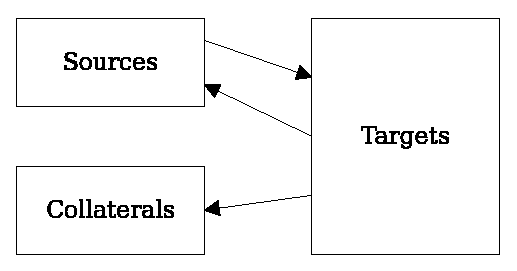
\includegraphics[scale=0.6]{figures/models/overview}}
   \caption{Structure of the reputation graph.}
   \label{fig:overview}
\end{figure}

The reputation of source nodes influences the reputation
of target nodes as much as the reputation of target nodes
influences the reputation of source nodes. Note that the
reputation of target nodes also influences the reputation of
collaterals, but the reputation of collaterals has no impact
in the reputation of sources and targets. The use of collaterals
allows us to isolate the impact of a set of arbitrary
nodes on the reputation graph if there is the need to do it, 
fixing reputation sources as the only set of nodes providing reputation. 

Given that the reputation of collaterals has no effect on
the reputation of nodes of other types, we can split the model
in two phases. In the first phase, we propagate the reputation
of the sources to the targets. In the second phase, we
propagate the reputation of the targets to the collaterals.

The reputation flows framework allows for different configurations.
In this work, we adopt research groups as reputation sources and publication 
venues as reputation targets, however collaterals (such as individual researchers) 
are absent from the ranking model, because we are only interested in calculating the 
P-scores of publication venues (weights of target nodes). Therefore, we do not need to
perform the second phase when calculating venue P-scores.


The interaction between reputation sources and reputation targets is inspired by the 
notion of {\em eigenvalue centrality} in complex 
networks~\cite{Brin1998,Langville2008,Langville2008,Newman2010}. 
In the reputation graph, if we consider only sources and targets, it is easy to 
identify reputation flows from sources to sources, from sources to targets, from 
targets to sources, and from targets to targets. These reputation flows can be 
modeled as a stochastic process. 
In particular, let $P$ be a \emph{right stochastic} %\footnote{A right stochastic matrix is ...} 
matrix of size $(|S|+|T|) \times (|S|+|T|)$ with the following structure: 

\newcommand{\bkt}[1]{ {^{\langle #1 \rangle}} }

\begin{align}\label{eq:newp}
%\[
P =
\left[
\begin{array}{r | r}
(d\bkt{S}) . P\bkt{SS}  & (1-d\bkt{S}) . P\bkt{ST} \\
\hline
(1-d\bkt{T}) . P\bkt{TS}  & (d\bkt{T}) . P\bkt{TT} \\
\end{array}
\right]
%\]
\end{align}
\noindent where each quadrant represents a distinct type of reputation flow, as follows: 

\begin{description}
\item $P\bkt{SS}$: right stochastic matrix of size $|S|\times |S|$ representing the 
transition probabilities between reputation sources;
\item $P\bkt{ST}$: matrix of size $|S|\times |T|$ representing the transition probabilities from reputation sources to targets;
\item $P\bkt{TS}$: matrix of size $|T|\times |S|$ representing the transition probabilities from reputation targets to sources;
\item $P\bkt{TT}$: right stochastic matrix of size $|T|\times |T|$ representing the transition probabilities between reputation targets.
\end{description}

The parameters $d\bkt{S}$, the fraction of reputation one wants to transfer among the source nodes themselves, 
and $d\bkt{T}$, the fraction of reputation one wants to transfer among the target nodes themselves,
control the relative importance of the reputation sources and targets. 
%These are useful parameters and the ability to set them is important to calibrate the impact of different reputation flows in the final score. 
If we do not want to consider reputation flows between nodes of the same type, it is sufficient to set both parameters to zero. If, instead, we want to consider reputation flows between nodes of the same type, we may increase these parameters according to the desired relative importance. Note that, as ($i$) the sub-matrices $P\bkt{SS}$ and $P\bkt{TT}$ are \emph{right stochastic}, ($ii$) each of the rows of matrices $P\bkt{ST}$ and $P\bkt{TS}$ sums to 1, and ($iii$) the parameters $d\bkt{S}$ and $d\bkt{T}$ are both in the range [0,1), then $P$ defines a Markov chain. Assuming that the transition matrix $P$ is ergodic, we can compute the steady state probability of each node 
and use it as a reputation score, the P-score. 
More formally, we can write: 
\begin{align}
\label{eq:ggP}
\gamma = \gamma P
\end{align}
where $\gamma$ is a row matrix with $|S|+|T|$ elements, 
where each row represents the transition probabilities of a node in the set $S\cup T$. 
%
This system of linear equations can be easily solved by standard Markov chain techniques. %TODO do we need to cite one?
Then, from Equation~\eqref{eq:ggP}, we obtain the steady state probabilities of all nodes in $S\cup T$, a.k.a. reputation sources and reputation targets.

\subsection{Flow Equations}\label{sec:flow-equations}

We recursively define the reputation of sources in terms of the reputation of targets, and the reputation of targets in terms of the reputation of sources. Specifically, the reputation $\gamma_s$ of a source $s$ is defined as:
\begin{align}
  \gamma_s = \sum_{t \in T} (1-d\bkt{T}).P_{ts}\bkt{TS} \gamma_t + \sum_{s' \in S} (d\bkt{S}).P_{s's}\bkt{SS} \gamma_{s'}\label{eqn:gs}
\end{align}
where $P_{ts}\bkt{TS}$ is the transition probability from $t$ to $s$, given by $P_{ts}\bkt{TS} = n_{ts} / n_t$, where $n_{ts}$ is the number of edges running from $t$ to $s$ and $n_t$ is the total number of edges running from $t$. Finally, $\gamma_t$ is the reputation of target $t$, defined recursively as:
\begin{align}
  \gamma_t = \sum_{s \in S} (1-d\bkt{S}).P_{st}\bkt{ST} \gamma_s + \sum_{t' \in T} (d\bkt{T}).P_{t't}\bkt{TT} \gamma_{t'}\label{eqn:gt}
\end{align}
where, similarly, $P_{st}\bkt{ST}$ is the transition probability from $s$ to $t$, given by $P_{st}\bkt{ST} = n_{st} / n_s$, where $n_{st}$ is the number of edges running from $s$ to $t$ and $n_s$ is the total number of edges running from $s$. 

% \subsection{Bipartite Reputation Graph}\label{sec:bipartite}

In our scenario, the reputation graph is as a bipartite graph. Therefore, the transition matrix $P$ is reduced to a periodic Markov chain with the following structure:
\begin{align}\label{eq:p}
%\[
P 
=
\left[
\begin{array}{c | c}
\bzr      &P\bkt{ST} \\
\hline
P\bkt{TS}  &\bzr    \\
\end{array}
\right]
\end{align}

From decomposition theory~\cite{meyer89}, we can obtain values for ranking the set of reputation {\em sources} by solving:
\begin{align}
\label{eq:top-rank}
\bgamma\bkt{S} = \bgamma\bkt{S} P'
\end{align}
\noindent where $P^\prime = P\bkt{ST} \times P\bkt{TS}$ is a stochastic matrix and $\bgamma\bkt{S}$ is a row matrix with $|S|$ elements, where each one represents the probability of a node in the set $S$ of reputation sources.
%
Note that matrix $P'$ has dimension $|S| \times |S|$ only and can be easily solved by standard Markov chain techniques.
Then, from Equation~\eqref{eq:venue-rank}, we obtain the reputation of all reputation \emph{targets} linked by the reputation sources:
\begin{align}
\label{eq:venue-rank}
\bgamma\bkt{T} = \bgamma\bkt{S} \times P\bkt{ST}
\end{align}

By modeling a scenario as a bipartite reputation graph instead of a general reputation graph, we reduce the network from a graph of size $(|S|+|T|)\times (|S|+|T|)$ to a graph of size $|S|\times |S|$, which allows us to compute the steady state probabilities more efficiently. %However, by using a bipartite graph, we are certainly losing some information, which may be critical for some applications. It is important to consider this trade-off when instantiating our framework. %conceptual framework of reputation flows. %When the information lost by not taking into account reputation flows directly from nodes of the same type, we should consider to adopt a bipartite reputation graph since it offers gains in efficiency. 


When there are collaterals, we can perform the second phase (propagation to collateral nodes) 
by further propagating the steady state probabilities of target nodes to the collateral set. 
In this case, we need a transition matrix $P\bkt{TC}$ of size $|T|\times |C|$ representing
the transitions from reputation targets to collaterals.

% \subsection{Reputation-based Ranking}\label{sec:ranking}
%
%The steady state probability of a node can be interpreted as its relative reputation, as transferred from other nodes in the reputation graph. Thus, we can directly use the value of this probability to rank reputation sources or reputation targets. Additionally, this probability can be further propagated to nodes we want to compare, which are in the collateral set. This propagation depends on a matrix $P\bkt{TC}$ of size $|T|\times |C|$ representing the transitions from reputation targets to collateral nodes. 
More generally, we can define the reputation score of an entity $e$ according to:
\begin{align}\label{eq:pscore}
  \text{P-score}(e) = \begin{cases}
	\sum_{t \in T} P_{te}\bkt{TC} \gamma_t & \text{if $e \in C$,}\\
    \gamma_e &\text{otherwise,}
  \end{cases}
\end{align}
\noindent where $P_{te}\bkt{TC}$ is the transition weight from a target node $t$ to a collateral node $e \in C$. The P-score of all candidate entities (targets or collaterals) can then be used to produce an overall reputation-oriented ranking of these entities.


\subsection{Instantiation Example}\label{sec:example}
% \subsection{Ranking Publication Venues} ?

The conceptual framework of reputation flows can be used in the academic context
to model the transference of reputation between research groups and 
publication venues by associating each type of reputation flow with a specific quadrant
of matrix $P$. That is:

\begin{align}\label{eq:newp}
%\[
P =
\left[
\begin{array}{r | r}
Group \rightarrow Group & Group \rightarrow Venue \\
\hline
Venue \rightarrow Group & Venue \rightarrow Venue \\
\end{array}
\right]
%\]
\end{align}

In this conceptual framework, research groups are 
aggregations of authors and publication venues are aggregations of papers.
In the first quadrant, the framework represents the reputation
flow from research groups to research groups, which can be expressed in
terms of co-authorship relations. In the second and 
third quadrants, the framework
represents group-venue and venue-group relations,
respectively. An author who publishes a paper somehow
transfers its own reputation to that paper or the converse,
a paper may transfer its reputation or acceptance by the
community to the authors who published it. In the fourth
quadrant, the framework represents the reputation flow between
venues, or between the papers in these venues. When a paper cites 
another, it is somehow
transferring part of its reputation to the cited paper. This
last quadrant is the focus of much more attention than the
other ones by the academic community. 

We should note that, while our network model allows modeling citations in the fourth quadrant, it is possible to compute 
steady state probabilities for the network without consideration to citations. This is accomplished by setting the parameter 
$d\bkt{T} = 0$. 
Thus, it should be clear that in all experiments described in this work, P-scores 
are computed without taking citations into account. 

Figure \ref{fig:ex1-MC} shows an example with two research groups used as reputation sources, Group 1 and Group 2, and three venues used as reputation targets, venues $\mbox{v}_1$, $\mbox{v}_2$ and $\mbox{v}_3$.
%
\begin{figure}[ht]
   %\centerline{\includegraphics[width=8cm]{figures/aggregation-b}}
   %\centerline{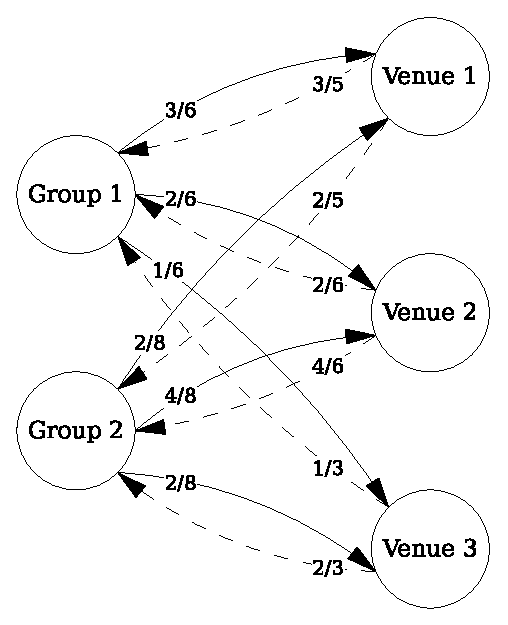
\includegraphics[width=5.5cm]{figures/models/bhrscore-w3}}
   \centerline{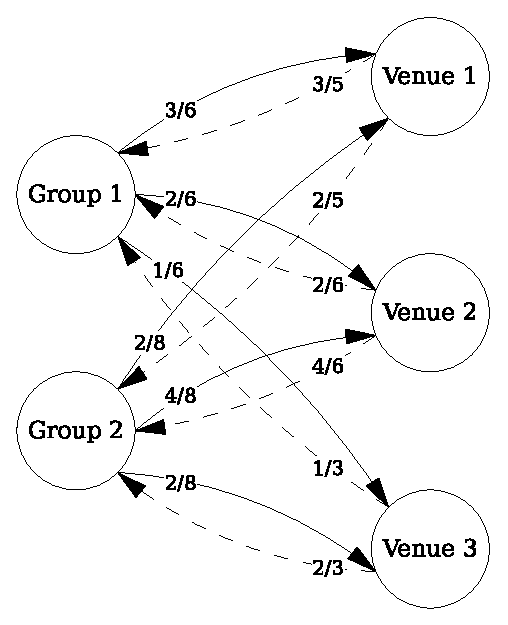
\includegraphics[width=5.2cm]{figures/models/bhrscore-w3}}
   \caption{Markov chain for an example with 2 research groups and 3 publication venues.}
   \label{fig:ex1-MC}
\end{figure}

From Figure \ref{fig:ex1-MC}, Group 1 published $3$ papers in venue $\mbox{v}_1$, $2$ papers in venue $\mbox{v}_2$, and $1$ paper in venue $\mbox{v}_3$. The number of publications of Group 1 is $6$. Venue $\mbox{v}_1$ receives $3$ papers of Group 1, and 2 papers of Group 2. The fractions of publications from groups to venues and from venues to groups are the edge weights. We have:
\[
P =
\left[
\begin{array}{c c | c c c }
0            &0             &3/6       &2/6         &1/6    \\
0            &0             &2/8       &4/8         &2/8    \\
\hline
3/5          &2/5           &0         &0           &0       \\
2/6          &4/6           &0         &0           &0       \\
1/3          &2/3           &0         &0           &0       \\
\end{array}
\right]
\]

This stochastic matrix corresponds to the Markov chain displayed in Figure~\ref{fig:ex1-MC}, which can be immediately aggregated to a two-state Markov chain, yielding:
%
\[
P^\prime = 
\left[
\begin{array}{c c }
0.467   &0.533 \\
0.400   &0.600
\end{array}
\right]
\]
\noindent which is the stochastic matrix we use in the solution of Equation (\ref{eq:top-rank}). (Recall that the dimension of $P^\prime$ is $T \times T$ and, as such, much smaller than that of $P$ for real size problems.) Solving Equation (\ref{eq:top-rank}) and applying Equation~\eqref{eq:venue-rank}, we obtain the ranking for the three venues: 
\begin{equation}
\bgamma\bkt{T} = \langle 0.36, 0.43, 0.21 \rangle
\end{equation}

Venue $\mbox{v}_2$ has the highest rank, followed by $\mbox{v}_1$, and then by $\mbox{v}_3$. We remark that the individual values give the {\em relative reputation} of each publication venue. 
%
Then, we can apply Equation (\ref{eq:pscore}) to compute the P-score of each entity in the reputation graph.


\subsection{Reputation Sources}
\label{sec:rep-sources}

The choice of the reputation sources is an important part of the method since 
its composition has a direct impact on the final rankings. 
There is no definitive way to make it. This choice depends on what we want to measure. 

One way to determine the top CS departments is through a simple randomization procedure.
It starts with all 126 research groups evaluated by the NRC \footnote{http://www.nap.edu/rdp/}
in its 2011 evaluation of CS graduate programs in the USA. 
First, we need to instantiate the model described previously with a single difference, 
a subset of 10 groups from the NRC evaluation is chosen randomly and used as reputation sources, while the remaining 116 groups
are used as reputation collaterals. This time we also need to execute the propagation of reputations 
from targets to collaterals with a transition matrix $P\bkt{TC}$ of size $|T|\times |C|$ that represents
relations from venues to the collateral research groups. This matrix can be built the same way
the $P\bkt{ST}$ (sources to targets) matrix is built, that is, by associating authors to research 
groups and their papers to publication venues and taking the relative number of papers published
in each venue as a transition probability.

Observe that the randomization procedure is only needed to
select the source nodes for the calculation of venue P-scores, it has no direct relation with the venue ranking
model described in the last section. A run of that procedure works as follows: 
\begin{enumerate}
\item Randomly select 10 departments from the set of top CS departments and use them as the set $s$ of reputation sources
\item Compute steady state probabilities for all nodes using the method described in the last section
\item Using the steady state probabilities of reputation collaterals as a score, select the 10 entities with 
highest scores and use them as a new set $s_{new}$ of reputation sources
\item If $s_{new} \not \equiv s$ then $s \leftarrow s_{new}$ and go back to step 1
\item $s_{auto} \leftarrow s_{new}$ 
\item Take $s_{auto}$ as the set of automatically selected reputation sources
\item Exit
\end{enumerate}

We repeated this procedure until the set of top 10 groups no longer changed.
By applying this randomization procedure 100 times to a set of 126 USA graduate programs, 
we ended up with a subset of 12 CS programs that appeared 
among the top 10 at least once, after the process stabilized. These 12 CS programs are
described in Table \ref{tab:departments}.

\begin{table}[ht!]
 \centering
 \begin{tabular}{l l} 
 \toprule
 \# & Department \\ 
 \midrule
 1  & Carnegie Mellon University \\
 2  & Georgia Institute of Technology \\
 3  & Massachusetts Institute of Technology \\
 4  & Stanford University \\
 5  & University of California-Berkeley \\
 6  & University of California-Los Angeles \\
 7  & University of California-San Diego \\
 8  & University of Illinois at Urbana-Champaign \\
 9  & University of Maryland College Park \\
 10 & University of Southern California \\
 11 & University of Michigan-Ann Arbor \\
 12 & Cornell University \\
 \bottomrule
 \end{tabular}
 \caption{Reputation sources obtained with the randomization procedure.}
 \label{tab:departments}
\end{table}

All the 12 departments above are among the top 5th percentile in the ranking produced by NRC. 
Moreover, the first 8 listed groups appeared among the top 10 at every single run.
This suggests that our recursive procedure is able to take advantage of patterns in the publication 
streams of the various CS departments to determine the most reputable ones in fully automatic fashion.
We further observe that this was done while setting the parameter $d\bkt{T} = 0$. That is, we did 
not use information on citation counts in the model. 

\subsection{Summary} 

The basic idea of the P-score metric is to associate a reputation with publication venues based on the publication patterns of 
a {\em reference set} of research groups in a given area or sub-area of knowledge. Given a pre-selected set of reference research groups, P-score associates weights with the publication venues the researchers in the reference groups publish in. Further, these weights can be used to rank other research groups or authors.

The reputation of a research group is strongly influenced by the reputation of its members, which is largely dependent on their publication records. We assume that:
\begin{enumerate}
\item A research group conveys reputation to a publication venue proportionally to its own reputation.
\item A publication venue conveys reputation to a research group proportionally to its own reputation.
\end{enumerate}

Once a reference group is selected, the reputation of its members is transferred to the venues. Recursively, since the reputation of research groups is correlated with the reputation of the venues in which they published, the venues transfer reputation to the groups. A score for venues can then be computed by solving a system of linear equations relating publication venues and research groups in the reputation graph, as exemplified in the section~\ref{sec:example}.


\section{Correlation with H-indices} 
\label{sec:correlation}

Bibliometric indicators can be roughly divided into two types. The attention indicators usually 
estimate researcher attention or the diffusion of a journal's articles through different 
forms of citation counts. 
The reputation indicators try to estimate a researcher's reputation based on the researcher's 
overall scientific production.
What we argue in this paper is that both perspectives have a complementary nature,
since indicators of different types are measuring similar but distinct aspects of
a journal's scientific relevance. 

We performed a combined analysis of conference rankings in Computer Science based on the H-index, an
attention indicator, and P-score, a reputation indicator. We chose the H-index as an attention 
indicator because of its popularity and availability in bibliometric search engines such as 
Google Scholar, Web of Science and Scopus. We chose P-score as a reputation indicator because 
of its ease of calculation and for being a good proxy for academic impact as shown by Ribas et 
al.~\cite{Ribas2015a}. 

The H-index~\cite{Hirsch2005} is a composite index of lifelong scientific contribution that takes 
into account the productivity of researchers and the citation impact of their publications.
A researcher has an H-index value of $ h $ if she has $ h $ publications that have been cited at 
least $ h $ times. For example, if a researcher has published 20 papers that received at least 20 
citations each, then her H-index is 20, assuming that 20 is the highest number for which the 
definition of the H-index holds. A journal's H-index can be computed 
in the same way by considering all publications and their collective citation data over a 
definite period as suggested by Braun et al.~\cite{Braun2006}.
Since the H-index was proposed in 2005, the original paper by~\cite{Hirsch2005} was 
cited 7,949 times, which attests to its popularity 
\footnote{According to Google Scholar, up to the end of 2017.}.

As any scientific impact index, the H-index has advantages and disadvantages. 
Some of its advantages are:

\begin{itemize}
\item The simplicity and intuitiveness of its formulation.
\item The longer citation time window when compared to impact factors.
\item H-index has a good predictive power regarding scientific achievement~\cite{Bornmann2005,Hirsch2007}.
\end{itemize}

H-index depends on citations to be calculated, thus it suffers from the 
same problems as any other citation-based indices. Some of its major disadvantages are:

\begin{itemize}
\item H-index does not distinguish citations from prestigious and peripheral journals, thus 
it measures popularity rather than quality.
\item The time to first citation can be very long.
\item It is not easy to collect all relevant information.
\item H-index is field-dependent~\cite{Wendl2007}.
\item Major sources do not always agree on its value~\cite{Bar-Ilan2008}. 
\end{itemize}

We propose to use P-score as a complementary index to deal with some of the problems
presented by citation-based indices such as the H-index.
P-score is a index of reputation among peers based on the publication pattern of a set of
reference groups of researchers, the reference seeds. It differs from other network-based 
indices because the venues' reputations derive exclusively from the reference seeds, which 
allows better control of the actual reputation flows. Additionally, to calculate P-scores we 
do not need citation data, which make P-scores easier to obtain than H-indices and avoids 
the problem of lack of data that arises from the long time to first citation.

We conducted experiments to investigate the relationship between P-scores and H-indices
in conference rankings. In particular, we wanted to estimate the degree of correlation between both 
indices. The data set consists of 794
Computer Science~\footnote{
While our data set is entirely composed of Computer Science conferences, nothing in our method is
particular to this field. That is, our index is applicable to any field of knowledge.
} 
conferences
for which the H5 index was available on Google Scholar~\footnote{https://scholar.google.com.br/}
in 2012. P-scores were calculated with
data obtained from DBLP \footnote{http://dblp.uni-trier.de/}. The reference set of research groups
was selected through the randomization process described in the previous section, 
yielding the 12 departments listed in Table \ref{tab:departments}.

\begin{figure}[ht]
\centering
  \begin{subfigure}{.475\linewidth}
  \centering
 
    \begin{tikzpicture} [scale=0.6]
      \begin{axis}[
          grid=major, % Display a grid
          grid style={dashed,gray!30}, % Set the style
          xlabel=Theoretical Z-Scores,
          ylabel=Sample Z-Scores,
          label style={font=\large},
          ymin=-3,
          ymax=10
        ]
        \addplot[blue, only marks, mark size=0.75pt] 
        table[x=zscore,y=hindex,col sep=comma] {data/normality.csv}; 

        \draw[dotted]
            (axis cs:\pgfkeysvalueof{/pgfplots/xmin},\pgfkeysvalueof{/pgfplots/xmin}) -- 
            (axis cs:\pgfkeysvalueof{/pgfplots/xmax},\pgfkeysvalueof{/pgfplots/xmax});
      \end{axis}
    \end{tikzpicture}
    \caption{H-index Normal Probability Plot}
    \label{fig:hindex_normality}
  \end{subfigure}
  ~
  \begin{subfigure}{.475\linewidth}
    \begin{tikzpicture} [scale=0.6]
      \begin{axis}[
          grid=major, % Display a grid
          grid style={dashed,gray!30}, % Set the style
          xlabel=Theoretical Z-Scores,
          ylabel=Sample Z-Scores,
          label style={font=\large},
          ymin=-3,
          ymax=10
        ]
        \addplot[blue, only marks, mark size=0.75pt] 
        table[x=zscore,y=pscore,col sep=comma] {data/normality.csv}; 

        \draw[dotted]
            (axis cs:\pgfkeysvalueof{/pgfplots/xmin},\pgfkeysvalueof{/pgfplots/xmin}) -- 
            (axis cs:\pgfkeysvalueof{/pgfplots/xmax},\pgfkeysvalueof{/pgfplots/xmax});
      \end{axis}
    \end{tikzpicture}
    % \caption{P-score}
    \caption{P-score Normal Probability Plot}
    \label{fig:pscore_normality}
  \end{subfigure}
\end{figure}

We first plotted normal probability plots for P-scores and H-indices in our conference data set 
to identify any departures from normality. A normal probability plot shows the theoretical Z-scores
according to the standard normal quantile function on the horizontal axis. For example, at the 90th
percentile (the value below which 90\% of the observations will fall), the normal distribution has a
Z-score of 1.28, meaning that the distribution value at this point is 1.28 standard deviations above the median value. On the vertical axis, if
we plot the Z-scores according to the quantile function described by our sample, we can verify
whether it is consistent with a sample from a normal distribution.

We compared theoretical and sample Z-scores for 794 quantiles (one for each data point) in Figures
\ref{fig:hindex_normality} and \ref{fig:pscore_normality}. The dotted line is the identity line for
which sample and theoretical Z-scores converge. As becomes clear from the plots, both distributions
are significantly skewed, indicating that P-scores and H-indices do not follow normal
distributions. This restricts the application of correlation measures such as Pearson's Product 
Moment Correlation in our analysis, since it requires that variables be approximately normally 
distributed. 

For this reason, we chose the Kendall-Tau coefficient to
study the correlation 
between H-index and P-score. It is a measure of rank
correlation that assumes a value between
-1 and 1. It is higher when observations have similar
ranks, assuming a value of 1
when two rankings are identical and -1 when they are the inverse of each other. 
A Kendall-Tau coefficient close to zero indicates
that both rankings are uncorrelated~\cite{Kendall1955,Baeza-Yates2011}.

\begin{figure}[ht]
\centering
  \begin{subfigure}{.475\linewidth}
  \centering
    \begin{tikzpicture} [scale=0.6]
      \begin{axis}[
          grid=major, % Display a grid
          grid style={dashed,gray!30}, % Set the style
          xlabel=P-score ranks,
          ylabel=H-index ranks
          xmin=-100,
          ymin=-100,
          xmax=900,
          ymax=900,
        ]
        \draw[red]
            (axis cs:0,0) -- 
            (axis cs:700.207670245,1000);
        \draw[red]
            (axis cs:0,0) -- 
            (axis cs:1000,700.207670245);
        \addplot[blue, only marks, mark size=0.75pt] 
        table[x=pscore,y=hindex,col sep=comma] {data/ranks.csv}; 

      \end{axis}
    \end{tikzpicture}
    \caption{Angle strategy for delimiting our three groups of interest: Top, Center and Bottom - with pivot at the origin.}
    \label{fig:angle_strategy}
  \end{subfigure}
  ~
  \begin{subfigure}{.475\linewidth}  
  \centering
    \begin{tikzpicture} [scale=0.6]
      \begin{axis}[
          grid=major, % Display a grid
          grid style={dashed,gray!30}, % Set the style
          xlabel=P-score ranks,
          ylabel=H-index ranks
          xmin=-100,
          ymin=-100,
          xmax=900,
          ymax=900,
        ]
        \draw[red]
            (axis cs:-100,-100) -- 
            (axis cs:700.207670245,1000);
        \draw[red]
            (axis cs:-100,-100) -- 
            (axis cs:1000,700.207670245);
        \addplot[blue, only marks, mark size=0.75pt] 
        table[x=pscore,y=hindex,col sep=comma] {data/ranks.csv}; 
  
      \end{axis}
    \end{tikzpicture}
    \caption{Angle strategy for delimiting our three groups of interest with pivot positioned behind the origin, at point (-100, -100).}
    \label{fig:angle_strategy_adapted}
  \end{subfigure}
\end{figure}

\begin{figure}[ht!]
  \begin{center}
    \begin{tikzpicture} 
      \begin{axis}[
          grid=major, % Display a grid
          grid style={dashed,gray!30}, % Set the style
          xlabel=P-score ranks,
          ylabel=H-index ranks,
          xmin=-100,
          ymin=-100,
          xmax=900,
          ymax=900,
          width=12cm,height=12cm
        ]
        \addplot[
          blue, only marks, mark size=0.75pt
        ] 
        table[x=pscore,y=hindex,col sep=comma] {data/ranks.csv}; 
        \addplot[
          red, only marks, mark size=0.75pt,
          nodes near coords*={\Label},
          visualization depends on={value \thisrow{label} \as \Label},
          style={font=\tiny}
        ] 
        table[x=pscore,y=hindex,col sep=comma] {data/ranks.csv}; 

      \end{axis}
    \end{tikzpicture}
    \caption{P-score VS H-index}
  \end{center}
\end{figure}

\begin{figure}[ht]
\centering
  \begin{subfigure}{.475\linewidth}
  \centering
    \begin{tikzpicture} [scale=0.6]
      \begin{axis}[
          grid=major, % Display a grid
          grid style={dashed,gray!30}, % Set the style
          xlabel=Norm. P-score ranks,
          ylabel=Norm. H-index ranks,
          xmin=-100,
          ymin=-100,
          xmax=900,
          ymax=900,
        ]
        \addplot[blue, only marks, mark size=0.75pt] 
        table[x=npscore,y=nhindex,col sep=comma] {data/ranks.csv}; 

      \end{axis}
    \end{tikzpicture}
    \caption{Normalized P-score VS H-index}
    \label{fig:angle_strategy}
  \end{subfigure}
  ~
  \begin{subfigure}{.475\linewidth}  
  \centering
    \begin{tikzpicture} [scale=0.6]
      \begin{axis}[
          grid=major, % Display a grid
          grid style={dashed,gray!30}, % Set the style
          xlabel=P-score ranks,
          ylabel=Total Citations ranks,
          xmin=-100,
          ymin=-100,
          xmax=900,
          ymax=900,
        ]
        \addplot[blue, only marks, mark size=0.75pt] 
        table[x=pscore,y=citations,col sep=comma] {data/ranks.csv}; 

      \end{axis}
    \end{tikzpicture}
    \caption{P-score VS Total Citations}
    \label{fig:angle_strategy}
  \end{subfigure}

  \begin{subfigure}{.475\linewidth}  
  \centering
    \begin{tikzpicture} [scale=0.6]
      \begin{axis}[
          grid=major, % Display a grid
          grid style={dashed,gray!30}, % Set the style
          xlabel=P-score ranks,
          ylabel=Citations Per Paper ranks,
          xmin=-100,
          ymin=-100,
          xmax=900,
          ymax=900,
        ]
        \addplot[blue, only marks, mark size=0.75pt] 
        table[x=pscore,y=perpaper,col sep=comma] {data/ranks.csv}; 

      \end{axis}
    \end{tikzpicture}
    \caption{P-score VS Citations Per Paper}
    \label{fig:angle_strategy}
  \end{subfigure}
  ~
  \begin{subfigure}{.475\linewidth}  
  \centering
    \begin{tikzpicture} [scale=0.6]
      \begin{axis}[
          grid=major, % Display a grid
          grid style={dashed,gray!30}, % Set the style
          xlabel=H-index ranks,
          ylabel=Citations ranks,
          xmin=-100,
          ymin=-100,
          xmax=900,
          ymax=900,
        ]
        \addplot[blue, only marks, mark size=0.75pt] 
        table[x=hindex,y=citations,col sep=comma] {data/ranks.csv}; 

      \end{axis}
    \end{tikzpicture}
    \caption{H-index VS Citations}
    \label{fig:angle_strategy}
  \end{subfigure}
\end{figure}

\begin{table}[ht!]
  \small
  \centering
  \begin{tabular}{llll} 
  \toprule
  First & Second & Kendall-Tau & Spearman \\ 
  \midrule
  P-score     & H-index           & 0.5153 & 0.6939 \\
  P-score     & Total Citations   & 0.5028 & 0.6751 \\
  P-score     & Citations/Paper   & 0.3894 & 0.5555 \\
  N. P-score  & N. H-index        & 0.4741 & 0.6507 \\
  H-index     & Total Citations   & 0.6141 & 0.7623 \\
  \bottomrule
  \end{tabular}
  \caption{Correlations between rankings}
  \label{tab:conferences}
\end{table}

Consider two conference rankings. Figure \ref{fig:pscore_hindex_ranks} shows the ranks of our 794 conferences according to
their P-scores
on the X-axis and their H-indices on the Y-axis. Points that are closer to the origin have better ranks (i.e. a data point at position 1 is better ranked than a data point at position 200).
The plot shows an evident correlation between the ranks that is confirmed
by a high Kendall-Tau of 0.5200259445. With a p-value smaller than 0.000001, we can safely reject the null 
hypothesis (that the rankings are uncorrelated) with a reasonable margin.

\section{Assessing conferences in CS}
\label{sec:notifications}

Since P-scores and H-indices are strongly correlated, most data points in our example are clustered close to the identity 
line, showing an apparent agreement between the indices. However, there are noticeable differences, 
particularly in those cases for which the P-score rank position is high and the H-index rank is low 
(top left corner of Figure \ref{fig:pscore_hindex_ranks}), or for which the H-index rank is high and the 
P-score rank is low (bottom right corner of Figure \ref{fig:pscore_hindex_ranks}). Therefore, we 
can distinguish between three groups of interest in the data set:

\begin{itemize}
\item \textit{Center Group}: highly correlated data points. These are the venues that are popular (i.e. high H-index) and reputable (i.e. high P-score), or venues that are unpopular and not very reputable.
\item \textit{Top Group}: venues with a high P-score and low H-index. These are the venues that are reputable (i.e. endorsed by researchers at top CS departments), but not very popular.
\item \textit{Bottom Group}: venues with a high H-index and low P-score. There are the venues that are popular, but not very reputable.

\end{itemize}


Next, we devise a strategy for delimiting the three sets
presented above. We draw two line segments, starting from
the origin, separated by an angle $ \theta $, and examine
how the Kendall-Tau coefficient for the data points in the 
Center Group varies with respect to variations in the angle 
$ \theta $. It is what we call the "angle strategy", as 
illustrated in Figure \ref{fig:angle_strategy}. We immediately 
notice several data points close to the origin
which are not included in the Center Group. This is a problem, 
given that these points correspond to CS conferences that have a high H-index rank and a high
P-score rank and thus, are strongly correlated. To
correct this, we move the point where the lines meet, which we also
refer to as the pivot, to a point behind the origin, one
such as (-100, -100), as illustrated in Figure \ref{fig:angle_strategy_adapted}. 
By doing so, we ensure that all data points near the origin are included in the
Center Group.

\begin{table}[ht!]
\centering
 \begin{tabular}{c c c c} 
 \toprule
 Angle & Kendall-Tau & Spearman & Items in center group \\ 
 \midrule
 90 & 0.5153 & 0.6939 & 794 \\ 
 80 & 0.5153 & 0.6939 & 794 \\
 70 & 0.5186 & 0.6989 & 793 \\
 60 & 0.5269 & 0.7094 & 790 \\
 50 & 0.5523 & 0.7341 & 777 \\
 40 & 0.5884 & 0.7611 & 749 \\
 30 & 0.6510 & 0.7998 & 689 \\
 20 & 0.7290 & 0.8295 & 576 \\
 10 & 0.8434 & 0.8481 & 345 \\
 \bottomrule
 \end{tabular}
 \caption{Angle strategy Kendall-Tau in center group by varying the angle.}
 \label{tab:angle_strategy}
\end{table}

Table \ref{tab:angle_strategy} describes how the Kendall-Tau coefficients vary for items 
in the Center Group, as we vary the angle $ \theta $, with the pivot positioned behind 
the origin as in Figure \ref{fig:angle_strategy_adapted}. We notice that for $ \theta = 20^{\circ} $, 
616 conferences are included in the Center
Group (close to 70\% of all conferences in the data set) and, that is accomplished with a very high Kendall-Tau 
coefficient (i.e. above 0.7). Thus, in our subsequent 
analysis, we employed the angle strategy with $ \theta = 20^{\circ} $, since it provides 
a good trade off between correlation and coverage in our data set.

\begin{table}[ht!]
  \small
  \centering
  \begin{tabular}{c c c c} 
  \toprule
  \# & Top & Center & Bottom \\ 
  \midrule
  1  & IROS      & ICRA        & IPTPS   \\
  2  & ICMCS     & CHI         & MOBIHOC \\
  3  & ISIT      & CVPR        & ACSAC   \\
  4  & ICCD      & AAAI        & ICWS    \\
  5  & CDC       & NIPS        & ISM     \\
  6  & ICPP      & DAC         & ISMIR   \\
  7  & WCNC      & ICASSP      & PIMRC   \\
  8  & LCPC      & STOC        & BIBE    \\
  9  & ISQED     & FOCS        & DFT     \\
  10 & ISER      & INTERSPEECH & FSKD    \\
  11 & WACV      & ICCAD       & ICIDS   \\
  12 & ITS       & IJCAI       & MMM     \\
  13 & ICWSM     & SODA        & ECIS    \\
  14 & AIED      & INFOCOM     & ISVLSI  \\
  15 & GIS       & ICML        & IHI     \\
  16 & CCCG      & ICIP        & MMVR    \\
  17 & DCC       & SIGMOD      & ARC     \\
  18 & HUMANOIDS & ICSE        & VNC     \\
  19 & LREC      & IPPS        & IAT     \\
  20 & WAFR      & ICCV        & ICAI    \\
  21 & WSDM      & ICDE        & ICA3PP  \\
  22 & CICC      & ACL         & ANALCO  \\
  23 & MMSP      & ECCV        & CNSR    \\
  24 & CLUSTER   & ISCA        & ICEBE   \\
  25 & CONLL     & KDD         & PAAP    \\
  26 & CLOUD     & SIGCOMM     & PROMAS  \\
  27 & MFCS      & SC          & WI      \\
  28 & FSR       & WWW         & WKDD    \\
  29 & ICAC      & ICDCS       & APSCC   \\
  30 & WABI      & DATE        & CATA    \\
  \bottomrule
  \end{tabular}
  \caption{Conferences (short names) ranked by P-score in the bottom, center and top groups.}
  \label{tab:conferences}
\end{table}

With the pivot positioned at (-100, -100) and $ \theta=30^{\circ} $, the Top Group ended with 127 conferences, the 
Center Group with 616 conferences, and the Bottom Group with 139 conferences. Table 
\ref{tab:conferences} presents the top 30 conferences, ranked by P-score, for each of our three groups.

The Center Group consists of conferences that have a high correlation between reputation and
popularity. The reputation of these conferences is well represented by the number of citations
they receive. This group represents conferences that are relatively easy to classify regarding
their scientific impact. Among them we find WWW, CVPR and KDD, to name a few.

The Top Group consists of conferences with a high P-score rank and low H-index rank. While these conferences
receive a relatively low number of citations, reputable researchers (i.e. our reference set of top researchers in Computer Science) still publish 
in them consistently, as we can observe from their high P-score ranks. The primary reason is that
conferences in the Top Group are usually venues associated with smaller subareas of Computer Science, and are therefore venues that receive a smaller
number of citations. Because of that, their H-indices tend to be smaller and their H-index rank positions tend to be worse. Despite that, many of these venues might have a high reputation in their subareas and thus, high P-scores. 
For example, ICPP, SPAA, LCPC and PPSC are conferences related to parallel processing that capture
considerable attention from the top CS departments, as we can observe from their high P-scores. However,
due to their modest H-indices, they may end up being neglected by funding councils and committees in
their assessment. The total number of publications in Parallel Processing is comparatively low 
compared to other subareas of Computer Science such as Algorithms or Database Management Systems~\cite{Hoonlor2013}. So, it is reasonable to assume that conferences 
in this subarea are expected to receive fewer citations than their counterparts in more popular subareas.
P-scores can assist human evaluators with funding decisions by shedding light on these conferences.

The Bottom Group consists of conferences with a low P-score rank and high H-index rank. These conferences
receive a high number of citations, but their reputation among top computer scientists is comparatively low, as reflected by their P-scores. Conferences in this
group are usually situated in the intersection between Computer Science and other areas of knowledge. Some examples of such venues are
ISMB, GECCO and PSB, which are related to Biocomputing, ISMIR, which is related to Music Information Retrieval, and
ISCAS, and VTC which are related to Engineering and Electronics. Because these are large research communities, venue H-indices tend to be 
relatively high (particularly with regard to Computer Science). In the case of these events, funding councils in Computer Science should consider not only the high H-indexes, but also the venue reputation among computer
scientists. Indeed, an exceptionally popular and reputable conference in electronics may not be as 
popular or prestigious when considering it from the point of view of computer scientists. That is, P-scores may aid 
human evaluators with funding decisions by pinpointing conferences that intersect multiple areas of knowledge and by providing
an estimate of the conference's reputation among peers in the field of interest.

\begin{table}[ht!]
  \small
  \centering
  \begin{tabular}{c c c c c} 
  \toprule
  \# & NLP & NN & ML & IR  \\ 
  \midrule
  1  & NIPS & NIPS & NIPS & SIGIR \\
  2  & ACL & ICML & ICML & CIKM \\
  3  & EMNLP & CVPR & CVPR & WWW \\
  4  & ICML & ICASSP & ECCV & SIGMOD \\
  5  & NAACL & ECCV & ICCV & VLDB \\
  6  & INTERSPEECH & AAAI & ICASSP & ICDE \\
  7  & CONLL & ICANN & BMVC & TREC \\
  8  & ICASSP & INTERSPEECH & IJCAI & WSDM \\
  9  & ICANN & UAI & AAAI & ECIR \\
  10 & IJCNN & ESANN & ICANN & KDD \\
  \bottomrule
  \end{tabular}
  \caption{Conferences (short names) ranked by P-score (top10 authors by MS Saliency) in four CS subareas: NLP, Art. NN, IR, and ML.}
  \label{tab:subareas-saliency}
\end{table}


\begin{table}[ht!]
  \small
  \centering
  \begin{tabular}{c c c c c} 
  \toprule
  \# & NLP & NN & ML & IR  \\ 
  \midrule
  1  & ACL & NIPS & NIPS & SIGIR \\
  2  & NAACL & ISNN & KDD & TREC \\
  3  & EMNLP & IJCNN & ICDM & CIKM \\
  4  & LREC & CDC & ICDE & ECIR \\
  5  & INTERSPEECH & ISCAS & ICML & WWW \\
  6  & COLING & ICML & SDM & WSDM \\
  7  & CONLL & ICRA & SIGMOD & RIAO \\
  8  & ICASSP & ADPRL & CIKM & NAACL \\
  9  & AAAI & IEEEISIC & VLDB & KDD \\
  10 & IWSLT & ICANN & UAI & CHI \\
  \bottomrule
  \end{tabular}
  \caption{Conferences (short names) ranked by P-score (top10 authors by MS H-Index) in four CS subareas: NLP, Art. NN, IR, and ML.}
  \label{tab:subareas-hindex}
\end{table}

\section{Conclusions}
\label{sec:conclusions}

We have compared the P-scores and H-indices of 794 conferences in Computer Science. 
We have found that P-scores and H-indices have a very high correlation reflected by a Kendall-Tau of 
approximately 0.52. However,
we have also found important differences between the two indices.
Our interpretation of these results are based on the intuition that while H-indices provide a quantification of the popularity of a publication or researcher among their peers, P-scores provide a quantification of the reputation of a publication or researcher among peers. We can then distinguish three separate cases. First, when P-scores and H-indices are strongly correlated, we have venues that are popular and of high reputation among computer scientists. Second, when P-scores are large (better rank position) and H-indices are small (worse rank position) we have venues of good reputation among computer scientists that are associated with small research communities or subareas. Third, when P-scores are small (worse rank position) and H-indices are large, we have venues of good popularity (usually associated with large research communities outside Computer Science) that do not count with high reputation among computer scientists (in the sense that they do not publish frequently there).
These differences indicate a complementary aspect to the indices. P-scores, used in conjunction with H-indices, allow distinguishing the three distinct types of venues mentioned above. This provides useful information which
can be employed
by research funding councils and committees to better understand 
the scientific relevance of venues and researchers and thus, take more informed funding decisions.

\bibliographystyle{spmpsci}
\bibliography{pscore_correlation}

\end{document}
